\documentclass[]{beamer}

\definecolor{computestgreen}{HTML}{AFBC20}

\mode<presentation>
{
    \usetheme{Berlin}
    \usecolortheme[named=computestgreen]{structure}
    \useoutertheme{miniframes}
    \useinnertheme{circles}
}

\usepackage[T1]{fontenc}
\usepackage[utf8]{inputenc}
\usepackage[dutch]{babel}
\usepackage{booktabs} % Pretty rules for tables
\usepackage{enumerate} % Enumerated lists
\usepackage{wrapfig} % Wrapping text around images
\usepackage{caption} % Advanced features for image/table captions

% Configure caption
\captionsetup{margin=10pt,font=scriptsize,labelfont=bf,labelsep=colon}

% For including images
\DeclareGraphicsExtensions{.pdf,.png,.jpg}
\graphicspath{{./images/}}

\title[Git]
{Git -- een introductie}

\author{Serrano Pereira}

\institute
{
  \inst{}
  Computest, Zoetermeer
}

\date{\today}

\subject{IT}

% Show ToC at beginning of each section
\AtBeginSubsection[]
{
  \begin{frame}<beamer>{Inhoud}
    \tableofcontents[currentsection,currentsubsection]
  \end{frame}
}

\begin{document}

% Title page
\frame{\titlepage}
\note{}

% ToC
\begin{frame}
\frametitle{Inhoud}
\tableofcontents
\end{frame}

\section{Over versiebeheer}

\subsection{Wat is ``versiebeheer''?}

\begin{frame}
    \begin{enumerate}
        \item Een systeem om versies van bestanden mee te registreren
        \item Auteur, datum, beschrijving, versie nummer
    \end{enumerate}
\end{frame}

\subsection{Waarom zou je het moeten gebruiken?}

\begin{frame}
    \begin{enumerate}
    \item Versies vergelijken
    \item Oude versies van bestanden opvragen
        \begin{itemize}
            \item Eerdere wijzigingen ongedaan maken
        \end{itemize}
    \item Terugzien wie een bepaalde wijziging heeft gemaakt
        \begin{itemize}
            \item Wanneer
            \item Waarom
        \end{itemize}
    \item Samenwerking
        \begin{itemize}
            \item Parallel aan de dezelfde bestanden werken
            \item Wijzigingen samenvoegen
        \end{itemize}
    \end{enumerate}
\end{frame}

\subsection{Waarvoor kan je het gebruiken?}

\begin{frame}
    \begin{enumerate}
        \item Tekst bestanden (bijv. broncode)
        \item Binaire bestanden (bijv. afbeeldingen)
    \end{enumerate}
\end{frame}

\subsection{Versiebeheersystemen}

\frame[plain]{
    \frametitle{Lokaal}

    \begin{figure}[h]
    \centering
    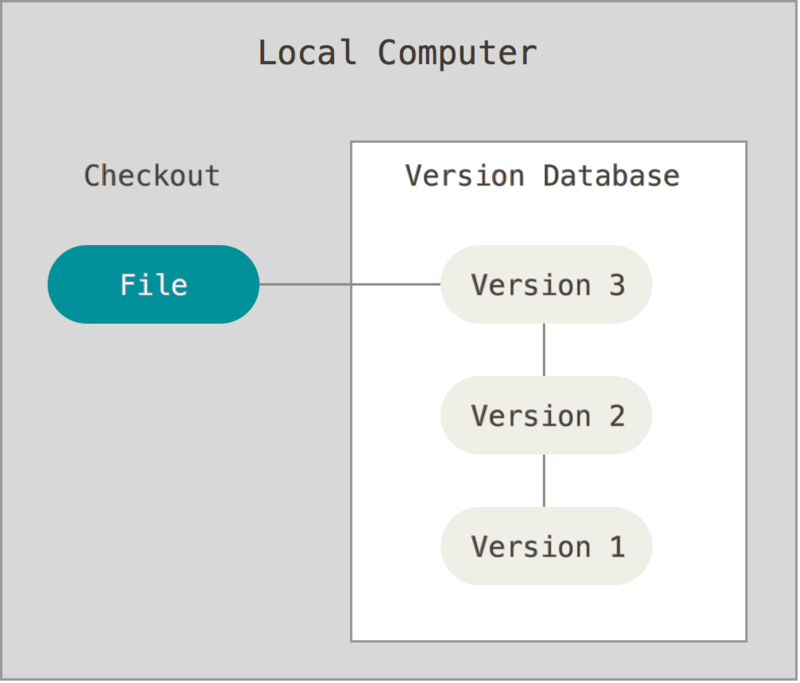
\includegraphics[width=\textheight]{local}
    \end{figure}
}

\frame[plain]{
    \frametitle{Gecentraliseerd}

    \begin{figure}[h]
    \centering
    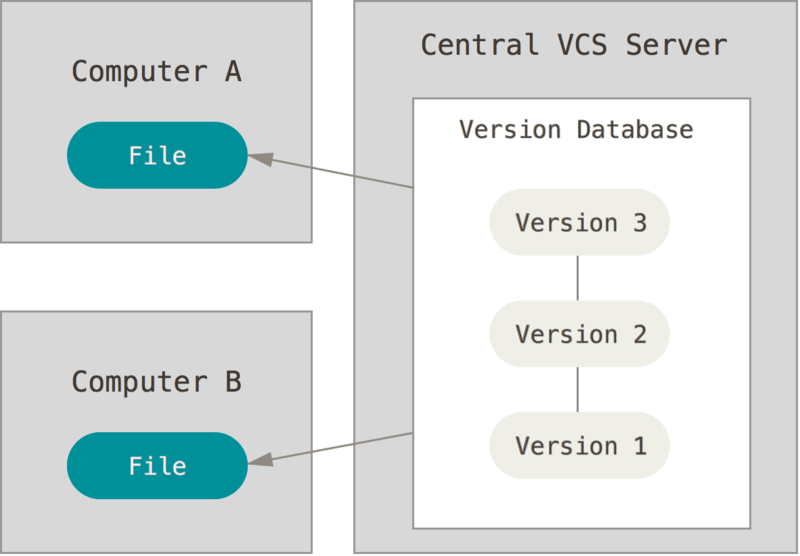
\includegraphics[width=\textheight]{centralized}
    \end{figure}
}

\begin{frame}
    \begin{itemize}
        \item \texttt{Concurrent Versions System (CVS)} (1986)
        \item \texttt{Subversion} (2000)
    \end{itemize}
\end{frame}

\frame[plain]{
    \frametitle{Gedistribueerd}

    \begin{figure}[h]
    \centering
    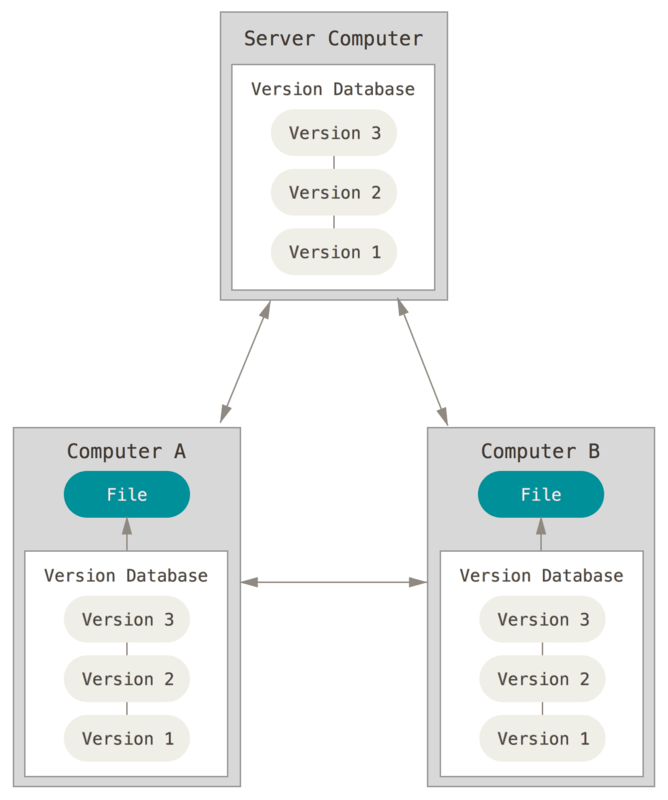
\includegraphics[width=0.8\textheight]{distributed}
    \end{figure}
}

\begin{frame}
    \begin{itemize}
        \item \texttt{BitKeeper} (2000)
        \item \texttt{Bazaar} (2005)
        \item \texttt{Git} (2005)
        \item \texttt{Mercurial} (2005)
    \end{itemize}
\end{frame}

\section{Git}

\subsection{Geschiedenis}

\frame[plain]{
    \begin{figure}[h]
    \centering
    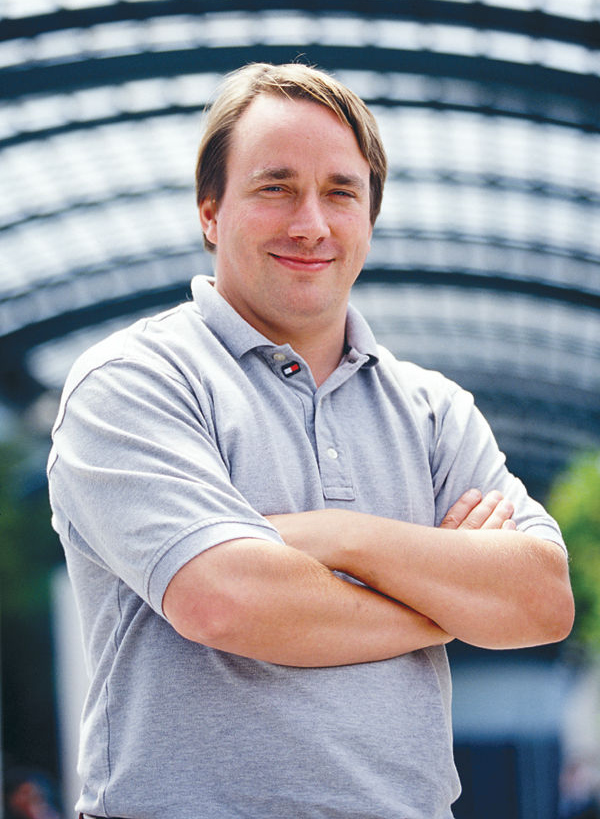
\includegraphics[width=0.7\textheight]{Linus_Torvalds}
    \end{figure}
}

\frame[plain]{
    \begin{figure}[h]
    \centering
    
\includegraphics[width=0.5\textheight]{Tux}
    \end{figure}
}

\frame[plain]{
    \begin{figure}[h]
    \centering
    
\includegraphics[width=0.5\textheight]{Git}
    \end{figure}
}

\subsection{Waarom Git?}

\begin{frame}
    \begin{itemize}
        \item Volledig gedistribueerd
        \item Goede ondersteuning voor niet-lineaire ontwikkeling
        \item Snelheid
        \item Efficiënt met grote projecten
        \item Gebruikersvriendelijk
    \end{itemize}
\end{frame}

\subsection{Hoe werkt het?}

\frame[plain]{
    \frametitle{Git denkt in momentopnames}

    \begin{figure}[h]
    \centering
    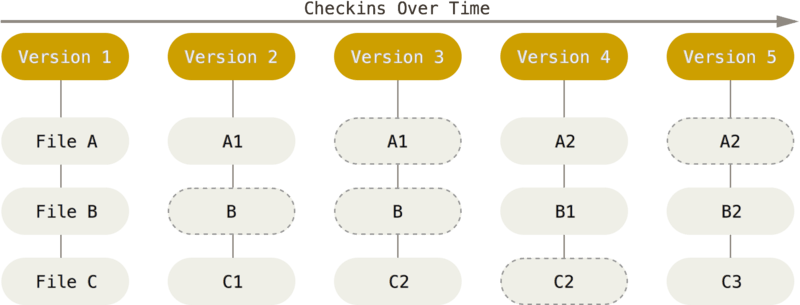
\includegraphics[width=\textwidth]{snapshots}
    \end{figure}
}

\frame[plain]{
    \frametitle{Integriteit}

    \begin{itemize}
        \item Alle objecten krijgen een controlegetal (checksum)
        \item SHA-1
    \end{itemize}

    \vspace{10 mm}
    \pause
    \centering
    \texttt{b40508769cb0aac22d9f73c8669c3a13f5e9cf0b}
}

\frame[plain]{
    \frametitle{De drie toestanden}

    \begin{figure}[h]
    \centering
    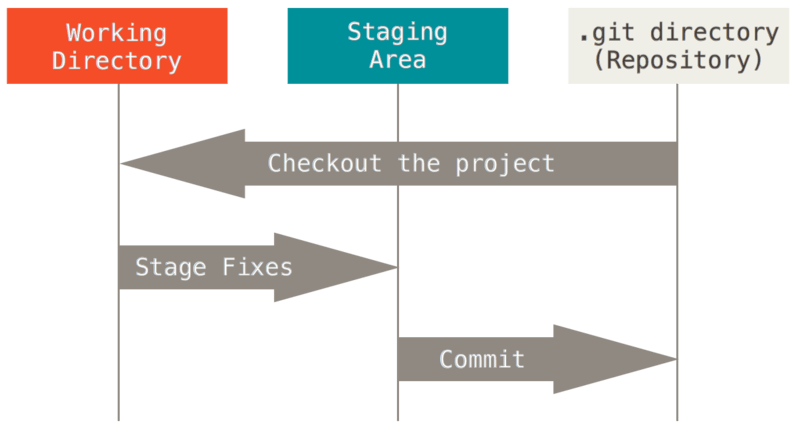
\includegraphics[width=\textwidth]{areas}
    \end{figure}
}

\begin{frame}
    \begin{itemize}
        \item De \texttt{git} commando-regel
        \begin{itemize}
            \item Geeft toegang to alle commando's
            \item Vereist basiskennis werken met Terminal
        \end{itemize}
        \pause
        \item Grafische tools
        \begin{itemize}
            \item Implementen maar een deel van de functionaliteit
        \end{itemize}
    \end{itemize}
\end{frame}

\section{Aan de slag}

\subsection{Installeren en configureren}

\begin{frame}
    \frametitle{Installeren}

    \centering

    \begin{block}{}
    \texttt{git}
    \end{block}

    \vspace{10 mm}
    \pause

    \url{https://git-scm.com/}
\end{frame}

\begin{frame}[fragile]
    \frametitle{Configureren voor gebruik}

    \begin{block}{}
\begin{verbatim}
git config --global user.name "John Doe"
git config --global user.email john@example.com
git config --global core.editor vim
git config --global color.diff true
\end{verbatim}
    \end{block}
\end{frame}

\section*{Naslagwerk}

\begin{frame}{Naslagwerk}
    \begin{itemize}
    \item Git website: \url{https://git-scm.com/}
    \item Pro Git book (gratis online boek): \url{https://git-scm.com/book/}
    \item Hoe schrijf je een goede Git Commit Message: \url{https://chris.beams.io/posts/git-commit/}
    \item Handige Git tips: \url{http://gitready.com/}
    \end{itemize}
\end{frame}

\end{document}
